\documentclass[border=5pt]{standalone}
\usepackage{tikz}
\usepackage{xcolor}
\usetikzlibrary{calc,shadows.blur}

% J3 - Orange torus/ring (donut shape)
\begin{document}
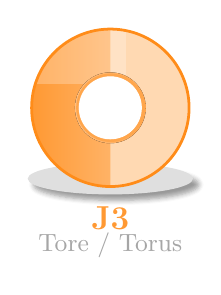
\begin{tikzpicture}

% Shadow
\fill[gray!25,blur shadow={shadow blur steps=5}] (0,-0.9) ellipse (1.05 and 0.2);

% Outer torus body (top view perspective)
% Outer ring shaded
\fill[left color=orange!80, right color=orange!40, middle color=orange!60]
  (0,0) circle (1.0);

% Inner hole (remove center)
\fill[white] (0,0) circle (0.42);

% 3D depth: bottom arc
\fill[orange!30] (0,-1.0) arc[start angle=-90, end angle=90, radius=1.0]
  -- (0,0.42) arc[start angle=90, end angle=-90, radius=0.42] -- cycle;

% Highlight arc on top-left
\begin{scope}
  \clip (0,0) circle (1.0);
  \fill[white,opacity=0.25] (-1.2,0.3) rectangle (0.2,1.1);
\end{scope}

% Inner edge shading
\fill[left color=orange!50, right color=orange!70] (0,0) circle (0.45);
\fill[white] (0,0) circle (0.40);

% Outline
\draw[orange!90, line width=1pt] (0,0) circle (1.0);
\draw[orange!70, line width=0.8pt] (0,0) circle (0.42);

% Label
\node[font=\bfseries\large, text=orange!80] at (0,-1.4) {J3};
\node[font=\small, text=gray!70] at (0,-1.75) {Tore / Torus};

\end{tikzpicture}
\end{document}
